\documentclass[twocolumn]{article}
\usepackage[top=15mm,bottom=15mm,left=15mm,right=15mm]{geometry}
\usepackage{amsmath,amssymb}
\usepackage{titlesec}
\usepackage{setspace}
\usepackage[dvipdfmx]{graphicx}
\usepackage{caption}
\setstretch{1.0}
\setlength{\parindent}{0pt}
\setlength{\parskip}{0pt}
\setlength{\abovedisplayskip}{3pt}
\setlength{\belowdisplayskip}{3pt}
\setlength{\abovedisplayshortskip}{3pt}
\setlength{\belowdisplayshortskip}{3pt}
\titlespacing*{\section}{0pt}{10pt}{5pt}
\titlespacing*{\subsection}{0pt}{8pt}{4pt}
\pagestyle{empty}

\begin{document}

\begin{enumerate}
  \item (a)の回路における電力の導出
        \begin{align*}
                & \text{入力電圧の最大値を} E_m \text{とすると}                          \\
          e     & = E_m \sin \omega t                                       \\
          i     & = \frac{e}{R} = \frac{E_m}{R} \sin \omega t               \\
          ei    & = E_m \sin \omega t \cdot \frac{E_m}{R} \sin \omega t     \\
                & = \frac{E_m^2}{R} \sin^2 \omega t                         \\
                & = \frac{E_m^2}{R} \left( 1 - \cos 2 \omega t \right)      \\
          E     & = \frac{E_m}{\sqrt{2}} \text{より,}                         \\
          E_m^2 & = 2E^2 \text{であるから,}                                      \\
          ei    & = ei_R = \frac{E^2}{R} \left( 1 - \cos 2 \omega t \right) \\
        \end{align*}

  \item (b)の回路における電力の導出
        \begin{align*}
          e              & = \sqrt{2}E \sin \omega t                                                                                               \\
                         & \text{インダクタンス } L\,[\text{H}] \text{ に流れる電流を } i\,[\text{A}]                                                            \\
                         & \text{とすると,誘導起電力 } e_L\,[\text{V}] \text{ は}                                                                            \\
          e_L            & = -L \frac{di}{dt}                                                                                                      \\
                         & e + e_L = 0 \text{ が成り立つため,}                                                                                            \\
          e              & = L \frac{di}{dt}                                                                                                       \\
          \frac{e}{L} dt & = di                                                                                                                    \\
          \int di        & = \int \frac{e}{L} dt                                                                                                   \\
          i              & = \int \left(\sqrt{2} E \sin \omega t dt\right)                                                                         \\
                         & = - \sqrt{2} \frac{E}{\omega L} \cos \omega t                                                                           \\
                         & = \sqrt{2}\frac{E}{\omega L}\sin \left(\omega t - \frac{\pi}{2}\right)                                                  \\
          ei             & = \frac{2E^2}{\omega L}\sin \omega t \cdot \sin \left(\omega t - \frac{\pi}{2}\right)                                   \\
                         & \text{積和の公式}                                                                                                            \\
                         & \sin\alpha \sin \beta = -\frac{1}{2} \left( \cos \left(\alpha + \beta\right) - \cos \left(\alpha - \beta\right) \right) \\
                         & \text{を用いて変形すると}                                                                                                        \\
          ei             & = \frac{2E^2}{\omega L} \left(- \frac{1}{2} \left(\cos\left(\omega t + \omega t - \frac{\pi}{2}\right) \right. \right.  \\
                         & \qquad\left.\left. - \cos\left(\omega t - \omega t + \frac{\pi}{2}\right)
          \right) \right)                                                                                                                          \\
                         & = -\frac{E^2}{\omega L} \cos \left(2\omega t - \frac{\pi}{2}\right)
        \end{align*}

  \item (c)の回路における電力の導出
        \begin{align*}
          e  & =\sqrt{2}E\sin\omega t                                   \\
             & \text{静電容量} C\,[\text{F}] \text{ に加わる電圧を } v\,[\text{V}] \\
             & \text{とすると,流れる電流 } i\,[\text{A}] \text{ は}               \\
          i  & = \frac{dq}{dt} = \frac{d}{dt}Cv                         \\
             & = C \frac{d \left(\sqrt{2}E\sin \omega t\right)}{dt}     \\
             & = \sqrt{2}\omega CE\cos\omega t                          \\
             & \text{これらから,電力eiは}                                       \\
          ei & = 2E^2 \omega C \sin\omega t \cos \omega t               \\
             & = E^2 \omega C \sin \left(2 \omega t\right)              \\
        \end{align*}

        \begin{center}
          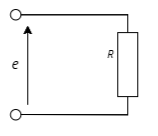
\includegraphics[width=0.6\linewidth]{./Circuits/Circuits_a.png}
          \captionof{figure}{回路a} % ✅ OK
        \end{center}
        \begin{center}
          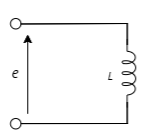
\includegraphics[width=0.6\linewidth]{./Circuits/Circuits_b.png}
          \captionof{figure}{回路b} % ✅ OK
        \end{center}
        \begin{center}
          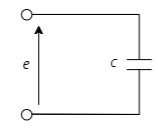
\includegraphics[width=0.6\linewidth]{./Circuits/Circuits_c.png}
          \captionof{figure}{回路c} % ✅ OK
        \end{center}

  \item (d)の回路における電力の導出
        \begin{align*}
          e    & =\sqrt{2}E\sin\omega t                                                                                                             \\
               & \text{また,各素子の電圧降下の合成と考えると}                                                                                                         \\
          e    & =iR + L \frac{di}{dt} \text{とも表すことができる.}                                                                                           \\
               & \text{抵抗とインダクタンスの合成インピーダンスを} Z \text{,}                                                                                            \\
               & \text{合成インピーダンスの位相のずれを} \Phi \text{とすると}                                                                                           \\
               & \text{電流} i \text{は,}                                                                                                              \\
          i    & = \frac{\sqrt{2}E}{\|Z\|} \sin \left( \omega t - \Phi\right)                                                                       \\
               & \text{この} i \text{を用いて電力} ei \text{を表すと,}                                                                                          \\
          ei   & = \sqrt{2}E\sin\omega t \cdot \frac{\sqrt{2}E}{\|Z\|} \sin \left( \omega t - \Phi\right)                                           \\
               & = \frac{2E^2}{\|Z\|}\sin\omega t \sin \left(\omega t - \Phi\right)                                                                 \\
               & \text{加法定理を用いて,}\sin \left(\omega t - \Phi\right) \text{を変形すると}                                                                    \\
          ei   & = \frac{2E^2}{\|Z\|}\sin\omega t \left(\sin\omega t \cos \Phi - \cos\omega t \sin \Phi\right)                                      \\
               & = \frac{2E^2}{\|Z\|} \left(\sin^2 \omega t \cos \Phi - \sin\omega t \cos\omega t \sin \Phi\right)                                  \\
               & = \frac{2E^2}{\|Z\|} \left(\sin^2 \omega t \cos \Phi \right) - \frac{2E^2}{\|Z\|} \left(\sin\omega t \cos\omega t \sin \Phi\right) \\
               & \text{左の項にはsinの半角公式}                                                                                                               \\
               & \text{右の項には} \sin \alpha \cos \beta \text{の積和公式を用いて変形すると}                                                                          \\
          ei   & = \frac{2E^2}{\|Z\|} \left(\left(\frac{1-\cos2\omega t}{2}\right)\cos \Phi\right)                                                  \\
               & - \frac{2E^2}{\|Z\|}\left(\frac{1}{2}\left(\sin2\omega t + \sin0\right) \sin \Phi\right)                                           \\
               & = \frac{E^2}{\|Z\|} \cos \Phi \left(1-\cos2\omega t\right) - \frac{E^2}{\|Z\|} \sin \Phi\sin2\omega t                              \\
               & \text{また,各素子における電力を求める.}                                                                                                           \\
               & \text{抵抗での電圧降下}e_R \text{は,}                                                                                                       \\
          e_R  & = iR = \frac{\sqrt{2}E}{\|Z\|} R \sin \left( \omega t - \Phi\right)                                                                \\
               & \text{であるから,}                                                                                                                      \\
          ei_R & = \frac{\sqrt{2}E}{\|Z\|} R \sin \left( \omega t - \Phi\right) \cdot \frac{\sqrt{2}E}{\|Z\|} \sin \left( \omega t - \Phi\right)    \\
               & = \frac{2E^2}{\|Z\|^2} R \sin^2 \left(\omega t - \Phi\right)                                                                       \\
               & \text{半角の公式を用いて}                                                                                                                   \\
               & = \frac{2E^2}{\|Z\|^2} R \left( \frac{1-\cos2\left(\omega t - \Phi\right)}{2} \right)                                              \\
               & = \frac{E^2}{\|Z\|^2} R \left( 1-\cos2\left(\omega t - \Phi\right)\right)                                                          \\
               & R\text{と}\omega L \text{との位相差は} \frac{\pi}{2} \text{であり,}                                                                          \\
               & \text{合成インピーダンス}Z\text{の位相差を}\Phi \text{とすると,}                                                                                     \\
        \end{align*}
        \begin{align*}
               & \frac{R}{\|Z\|} = \cos \Phi \text{となるため,}                                                                                           \\
          ei_R & = \frac{E^2}{\|Z\|} \cos \Phi \left( 1-\cos2\left(\omega t - \Phi\right)\right)                                                     \\
               & \text{次にコイルでの電圧降下}e_L \text{は,}                                                                                                     \\
          e_L  & = L \frac{di}{dt} = L \frac{d}{dt} \left( \frac{\sqrt{2}E}{\|Z\|} \sin \left( \omega t - \Phi\right) \right)                        \\
               & = \frac{\sqrt{2}E}{\|Z\|} \omega L \cos \left(\omega t - \Phi\right)                                                                \\
               & \text{であるから,}                                                                                                                       \\
          ei_L & = \frac{\sqrt{2}E}{\|Z\|}\omega L \cos\left(\omega t - \Phi\right) \cdot \frac{\sqrt{2}E}{\|Z\|} \sin \left( \omega t - \Phi\right) \\
               & = \frac{2E^2}{\|Z\|^2} \omega L \cos\left(\omega t - \Phi\right)\sin\left(\omega t - \Phi\right)                                    \\
               & \text{積を和に直す公式を用いて変形すると,}                                                                                                           \\
          ei_L & = \frac{2E^2}{\|Z\|^2}\omega L \left(\frac{1}{2} \left(\sin 2\omega t - 2\Phi\right)\right)                                         \\
               & = \frac{E^2}{\|Z\|^2}\omega L \left(\sin 2\omega t - 2\Phi\right)                                                                   \\
               & \text{また,} \frac{\omega L}{\|Z\|} = \sin \Phi \text{となるため,}                                                                         \\
          ei_L & = \frac{E^2}{\|Z\|}\sin \Phi \left(\sin 2\omega t - 2\Phi\right)                                                                    \\
        \end{align*}

        \begin{center}
          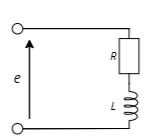
\includegraphics[width=0.6\linewidth]{./Circuits/Circuits_d.png}
          \captionof{figure}{回路d} % ✅ OK
        \end{center}

  \item (e)の回路における電力の導出
        \begin{align*}
          e & =\sqrt{2}E\sin\omega t      \\
            & \text{並列接続であるから,抵抗および}      \\
            & \text{インダクタンスにかかる電圧は等しいので,} \\
          e & = e_R = e_L                 \\
            & \text{また,各素子における電圧降下で考えると,} \\
          e & = {i_R}R = L\frac{di_L}{dt} \\
        \end{align*}

        \begin{align*}
                        & \text{抵抗に流れる電流は,オームの法則より,}                                                                                                      \\
          i_R           & = \frac{e}{R}                                                                                                                   \\
                        & = \frac{\sqrt{2}E}{R}\sin \omega t                                                                                              \\
                        & \text{インダクタンスに流れる電流は,}                                                                                                          \\
          e             & = L\frac{di_L}{dt}                                                                                                              \\
          \frac{e}{L}dt & = di_L                                                                                                                          \\
          \int di_L     & = \int \frac{e}{L}dt                                                                                                            \\
          i_L           & = \frac{\sqrt{2}E}{L} \int \sin \omega t dt                                                                                     \\
                        & = -\frac{\sqrt{2}E}{\omega L} \cos \omega t                                                                                     \\
                        & \text{ところで,合成アドミタンス}Y\text{は,}                                                                                                  \\
          Y             & = \frac{1}{R} + \frac{1}{j\omega L}                                                                                             \\
                        & = \frac{1}{R} - j\frac{1}{\omega L}                                                                                             \\
          \|Y\|         & = \sqrt{{\left(\frac{1}{R}\right)}^2 + {\left(\frac{1}{\omega L}\right)}^2}                                                     \\
                        & \text{つまり,合成インピーダンス}Z\text{は,}                                                                                                  \\
          \|Z\|         & = \frac{\omega LR}{\sqrt{R^2 + {\left(\omega L\right)}^2}}                                                                      \\
                        & \text{電圧を基準として電流の位相差をを考えると,}                                                                                                    \\
                        & \text{電圧と同位相である}\frac{1}{R}\text{と,}-\frac{\pi}{2}\text{ずれている}\frac{1}{\omega L}                                                \\
                        & \text{によって得られる電流は}Y\text{の位相であるため,}                                                                                             \\
                        & \text{Yの位相を}\Phi\text{とすると,}                                                                                                    \\
                        & \cos \Phi = \frac{\frac{1}{R}}{\|Y\|} = \frac{\|Z\|}{R} \Rightarrow  \frac{1}{R} = \frac{\cos \Phi}{\|Z\|}                      \\
                        & \sin \Phi = \frac{\frac{1}{\omega L}}{\|Y\|} = \frac{\|Z\|}{\omega L} \Rightarrow  \frac{1}{\omega L} = \frac{\sin \Phi}{\|Z\|} \\
                        & \text{となる.これらから電流}i_R\text{と,}i_L\text{を変形すると,}                                                                                 \\
          i_R           & = \frac{\sqrt{2}E}{R}\sin \omega t                                                                                              \\
                        & = \frac{\sqrt{2}E}{\|Z\|}\cos \Phi \sin \omega t                                                                                \\
          i_L           & = -\frac{\sqrt{2}E}{\omega L} \cos \omega t                                                                                     \\
                        & = -\frac{\sqrt{2}E}{\|Z\|} \sin \Phi \cos \omega t                                                                              \\
                        & \text{となり,式3.17,式3.18が得られ,各素子の電力は,}                                                                                             \\
        \end{align*}
        \begin{align*}
          ei_R            & = \sqrt{2}E\sin\omega t \cdot \frac{\sqrt{2}E}{\|Z\|}\cos\Phi\sin\omega t                     \\
                          & = \frac{2E^2}{\|Z\|}\cos\Phi\sin^2\omega t                                                    \\
                          & \text{半角の公式を用いて,}                                                                             \\
                          & = \frac{2E^2}{\|Z\|}\cos\Phi\left(\frac{1 - \cos 2\omega t}{2}\right)                         \\
                          & = \frac{E^2}{\|Z\|}\cos\Phi\left(1 - \cos 2\omega t\right)                                    \\
          ei_L            & = \sqrt{2}E\sin\omega t \cdot \left(-\frac{\sqrt{2}E}{\|Z\|} \sin \Phi \cos \omega t \right)  \\
                          & = \frac{2E^2}{\|Z\|} \sin\Phi \sin\omega t\cos\omega t                                        \\
                          & \text{積和の公式を用いて,}                                                                             \\
                          & = \frac{2E^2}{\|Z\|}\sin\Phi \left( \frac{1}{2} \left(\sin 2\omega t - \sin 0 \right) \right) \\
                          & = \frac{E^2}{\|Z\|}\sin\Phi\sin 2\omega t                                                     \\
          \therefore ei_R & = \frac{E^2}{\|Z\|}\cos\Phi\left(1 - \cos 2\omega t\right)                                    \\
          \therefore ei_L & = \frac{E^2}{\|Z\|}\sin\Phi\sin 2\omega t                                                     \\
        \end{align*}

  \item (f)の回路における電力の導出
        \begin{align*}
          e             & = \sqrt{2}E\sin\omega t                                                                               \\
                        & \text{ここで,各素子の合成インピーダンスを考える.}                                                                         \\
          Z_{R1}        & = R_1                                                                                                 \\
          Z_{RL}        & = R_2 + j\omega L                                                                                     \\
                        & \text{であるから,並列接続部分の合成インピーダンスは,}                                                                       \\
          \frac{1}{Z_p} & = \frac{1}{Z_{R1}} + \frac{1}{Z_{RL}}                                                                 \\
                        & \text{回路全体の合成インピーダンスを}Z\text{とすると,}                                                                   \\
          Z             & = R_0 + Z_p                                                                                           \\
                        & Z\text{の位相を}\Phi\text{とすると,回路に流れる電流}i_s\text{は,}                                                      \\
          i_s           & = \frac{\sqrt{2}E}{\|Z\|}\sin\left(\omega t - \Phi\right)                                             \\
                        & \text{となり,電力は}                                                                                        \\
          ei            & = \sqrt{2}E\sin\omega t \cdot \frac{\sqrt{2}E}{\|Z\|}\sin\left(\omega t - \Phi\right)                 \\
                        & = \frac{E^2}{\|Z\|} \cos \Phi \left(1-\cos2\omega t\right) - \frac{E^2}{\|Z\|} \sin \Phi\sin2\omega t \\
                        & \text{また,各素子の電力は,その素子に流れる電流,}                                                                         \\
                        & \text{その素子にかかる電圧,その素子のインピーダンスに}                                                                       \\
                        & \text{よって立式されている.}                                                                                    \\
        \end{align*}

  \item (g)の回路における電力の導出
        \begin{align*}
          e             & = \sqrt{2}E\sin\omega t \text{とする.}                                                                                     \\
                        & \text{直列接続であるから合成インピーダンス}Z\text{は,}                                                                                     \\
          Z             & = R + \frac{1}{j\omega C} = R -j\frac{1}{\omega C}                                                                      \\
                        & \text{となり,}                                                                                                             \\
          \|Z\|         & = \sqrt{R^2 + {\left( \frac{1}{\omega C} \right)}^2}                                                                    \\
                        & Z\text{による位相のずれを}\Phi\text{とすると,}                                                                                       \\
                        & \text{コンデンサによって電流は電圧よりも位相が}                                                                                             \\
                        & \text{進むため,}                                                                                                            \\
          i             & = \frac{e}{\|Z\|} = \frac{\sqrt{2}E}{\|Z\|}\sin\left(\omega t + \Phi\right)                                             \\
                        & \text{これらから,回路全体の電力は,}                                                                                                  \\
          ei            & = \sqrt{2}E\sin\omega t \cdot \frac{\sqrt{2}E}{\|Z\|}\sin\left(\omega t + \Phi\right)                                   \\
                        & = \frac{2E^2}{\|Z\|}\sin\omega t\sin\left(\omega t + \Phi\right)                                                        \\
                        & \text{加法定理を用いて変換すると,}                                                                                                   \\
                        & = \frac{2E^2}{\|Z\|}\sin\omega t\left(\sin\omega t \cos \Phi + \cos\omega t \sin \Phi\right)                            \\
                        & = \frac{2E^2}{\|Z\|}\left(\sin^2\omega t \cos \Phi + \sin\omega t\cos\omega t \sin \Phi\right)                          \\
                        & \text{半角公式および,積和公式を用いれば,}                                                                                               \\
          \therefore ei & = \frac{E^2}{\|Z\|}\left(\left(1-\cos2\omega t\right)\cos \Phi + \sin2\omega t \sin \Phi\right)                         \\
                        & \text{次に}e_R\text{について考える.}e_R\text{は,オームの法則より,}                                                                        \\
          e_R           & = iR = \frac{\sqrt{2}ER}{\|Z\|}\sin\left(\omega t + \Phi\right)                                                         \\
          ei_R          & = \frac{\sqrt{2}ER}{\|Z\|}\sin\left(\omega t + \Phi\right)\cdot \frac{\sqrt{2}E}{\|Z\|}\sin\left(\omega t + \Phi\right) \\
                        & = \frac{2E^2R}{{\|Z\|}^2}\sin^2\left(\omega t + \Phi\right)                                                             \\
                        & = \frac{2E^2R}{{\|Z\|}^2}\left(\frac{1 - \cos2\left(\omega t + \Phi\right)}{2}\right)                                   \\
                        & = \frac{E^2R}{{\|Z\|}^2}\left(1 - \cos2\left(\omega t + \Phi\right)\right)                                              \\
                        & \text{ここで,}\frac{R}{\|Z\|} = \cos \Phi\text{であるから,}                                                                     \\
                        & = \frac{E^2}{{\|Z\|}}\cos\Phi\left(1 - \cos2\left(\omega t + \Phi\right)\right)                                         \\
        \end{align*}
        \begin{align*}
            &\text{次にキャパシタンスによる電力を考える.}\\
            i &= \frac{de_c}{dt}C\\
            \frac{1}{C} i dt &= de_c\\
            \int de_c &= \int \frac{1}{C} i dt\\
            e_c &=  \frac{1}{C} \int \frac{\sqrt{2}E}{\|Z\|} \sin\left(\omega t + \Phi\right)dt\\
            e_c &=  \frac{\sqrt{2}E}{C \|Z\|} \int \sin\left(\omega t + \Phi\right)dt\\
            e_c &=  -\frac{\sqrt{2}E}{\omega C \|Z\|} \cos\left(\omega t + \Phi\right)\\
            ei_c  &= -\frac{\sqrt{2}E}{\omega C \|Z\|} \cos\left(\omega t + \Phi\right) \cdot \frac{\sqrt{2}E}{\|Z\|}\sin\left(\omega t + \Phi\right)\\
                  &= -\frac{2E^2}{\omega C {\|Z\|}^2} \cos\left(\omega t + \Phi\right) \sin\left(\omega t + \Phi\right)\\
                  &\sin\Phi = \frac{\frac{1}{\omega C}}{\|Z\|} = \frac{1}{\omega C \|Z\|} \text{及び,加法定理の逆より,}\\
\therefore ei_c   &= -\frac{E^2}{\|Z\|} \sin2\left(\omega t + \Phi\right)\\
        \end{align*}

        \begin{center}
            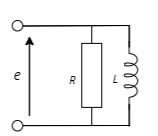
\includegraphics[width=0.4\linewidth]{./Circuits/Circuits_e.png}
            \captionof{figure}{回路e} % ✅ OK
          \end{center}
          \begin{center}
            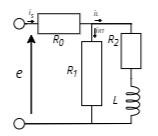
\includegraphics[width=0.4\linewidth]{./Circuits/Circuits_f.png}
            \captionof{figure}{回路f} % ✅ OK
          \end{center}
          \begin{center}
            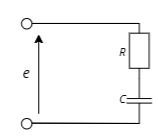
\includegraphics[width=0.4\linewidth]{./Circuits/Circuits_g.png}
            \captionof{figure}{回路g} % ✅ OK
          \end{center}

        \begin{center}
          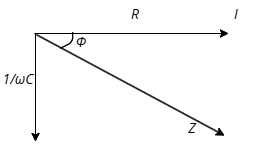
\includegraphics[width=0.5\linewidth]{./capacitor_Vector_img.png}
          \captionof{figure}{ベクトル図} % ✅ OK
        \end{center}

  \item (h)の回路における電力の導出
        \begin{align*}
          e               & = \sqrt{2}E\sin\omega t                                                                 \\
                          & \text{合成アドミタンスは,}                                                                       \\
          Y               & = \frac{1}{R} + \frac{1}{\frac{1}{j\omega C}}                     \\
                          & = \frac{1}{R} + j\omega C                            \\
          \|Y\|           & = \sqrt{{\left(\frac{1}{R}\right)}^2 + {\left(\omega C\right)}^2} \\
          \|Z\|           & = \frac{1}{\|Y\|}                                                                       \\
          & \text{並列接続より各素子にかかる電圧は等しい.}                                                             \\
          i_R             & = \frac{e}{R}                                                                           \\
          ei_R            & = \sqrt{2}E\sin\omega t \cdot \frac{\sqrt{2}E}{R}\sin\omega t                           \\
                          & = \frac{2E^2}{R}\sin^2 \omega t                                                         \\
                          & = \frac{E^2}{R}\left(1 - \cos 2 \omega t\right)                                         \\
                          & \text{ここで,合成アドミタンスとの位相差を考えると}                                                           \\
                          & \frac{\frac{1}{R}}{\|Y\|} = \frac{\|Z\|}{R} = \cos \Phi\text{であるから,}                    \\
          \therefore ei_R & = \frac{E^2}{\|Z\|}\cos \Phi\left(1 - \cos 2 \omega t\right)\\
          &\text{次にキャパシタンスによる電力を考える.}     \\
          i_c &= \frac{de_c}{dt}C\\
              &= C\frac{d}{dt}\left(\sqrt{2}E\sin\omega t\right)\\
              &= \sqrt{2}E \omega C  \cos\omega t\\
        ei_c  &= \sqrt{2}E\sin\omega t \cdot \sqrt{2}E \omega C  \cos\omega t\\
              &= 2E^2 \omega C \sin\omega t \cos\omega t\\
              &= E^2 \omega C \sin2\omega t\\
        \end{align*}
        \begin{align*}
            &\text{ここで,電圧を基準にしてベクトルを考えると,}\\
            &\text{位相差}\Phi\text{を使って,}\\
            \sin \Phi &= \frac{\omega C}{\|Y\|} = \|Z\|\omega C\\
            \omega C &= \frac{1}{\|Z\|} \sin \Phi\text{であるから}\\
\therefore ei_c &= \frac{E^2}{\|Z\|} \sin\Phi \sin2\omega t\\
        \end{align*}

  \item (i)の回路における電力の導出
        \begin{align*}
          e               & = \sqrt{2}E\sin\omega t\text{とする.}                                                                                                       \\
                          & \text{合成インピーダンスは}                                                                                                                        \\
          Z               & = R + j\omega L + \frac{1}{j\omega C}                                                                                                    \\
                          & = R + j\omega L -j \frac{1}{\omega C}                                                                                                    \\
          \|Z\|           & = \sqrt{R^2 + j{\left(\omega L - \frac{1}{\omega C}\right)}^2}                                                                           \\
                          & \text{合成インピーダンスの位相差を}\Phi\text{とする.}                                                                                                     \\
                          & \text{電流はオームの法則より,}                                                                                                                      \\
          i               & = \frac{e}{\|Z\|}                                                                                                                        \\
                          & = \frac{\sqrt{2}E}{\|Z\|}\sin \left(\omega t - \Phi\right)                                                                               \\
          ei              & = \sqrt{2}E\sin\omega t \cdot \frac{\sqrt{2}E}{\|Z\|}\sin \left(\omega t - \Phi\right)                                                   \\
                          & = \frac{2E^2}{\|Z\|}\sin\omega t  \sin \left(\omega t - \Phi\right)                                                                      \\
                          & \text{加法定理より,}                                                                                                                           \\
                          & = \frac{2E^2}{\|Z\|}\sin\omega t \left( \sin \omega t \cos \Phi - \cos \omega t \sin \Phi \right)                                        \\
                          & = \frac{2E^2}{\|Z\|} \left( \sin^2\omega t \cos \Phi - \sin \omega t \cos \omega t \sin \Phi \right)                                     \\
                          & = \frac{2E^2}{\|Z\|} \left( \frac{1 - \cos 2 \omega t}{2} \cos \Phi - \frac{1}{2} \left( \sin2\omega t  + \sin 0\right)\sin \Phi \right) \\
          \therefore ei   & = \frac{E^2}{\|Z\|} \cos \Phi \left(1-\cos2\omega t\right) - \frac{E^2}{\|Z\|} \sin\Phi \sin 2 \omega t                                  \\
          ei_r            & = i^2 R = \frac{2E^2}{(\|Z\|)^2}R\sin^2\left(\omega t -\Phi\right)                                                                       \\
                          & \frac{R}{\|Z\|} = \cos \Phi\text{より,}                                                                                                    \\
                          & = \frac{2E^2}{\|Z\|} \cos \Phi \sin^2\left(\omega t - \Phi\right)                                                                        \\
                          & = \frac{2E^2}{\|Z\|} \cos \Phi \left( \frac{1 - \cos 2 \left(\omega t - \Phi\right)}{2} \right)                                          \\
          \therefore ei_r & = \frac{E^2}{\|Z\|} \cos \Phi \left( 1 - \cos 2 \left(\omega t - \Phi\right)\right)                                                      \\
                          & \text{次に,インダクタンスでの電力を考える.}
        \end{align*}
        \begin{align*}
          e_L             & = L \frac{di}{dt} = L \frac{d}{dt} \left( \frac{\sqrt{2}E}{\|Z\|}\sin \left( \omega t - \Phi\right)\right)                          \\
                          & = \frac{\sqrt{2}E}{\|Z\|}\omega L \cos \left(\omega t - \Phi\right)                                                                 \\
          ei_L            & = \frac{\sqrt{2}E}{\|Z\|}\omega L \cos \left(\omega t - \Phi\right) \cdot \frac{\sqrt{2}E}{\|Z\|}\sin \left( \omega t - \Phi\right) \\
                          & = \frac{2E^2}{{\|Z\|^2}}\omega L \sin \left(\omega t - \Phi\right) \cos \left(\omega t - \Phi\right)                                \\
                          & = \frac{2E^2}{{\|Z\|}^2}\omega L \left(\frac{1}{2}\sin2\left(2\omega t\right)\right)                                                \\
          \therefore ei_L & = \frac{E^2}{{\|Z\|}^2}\omega L \sin2\left(\omega t - \Phi\right)                                                                   \\
                          & \text{最後にキャパシタンスの電力を考える.}                                                                                                           \\
          i               & = \frac{de_C}{dt}C                                                                                                                  \\
          \int de_C       & = \frac{1}{C} \int i dt                                                                                                             \\
          de_C            & = \frac{1}{C} \int \frac{\sqrt{2}E}{\|Z\|}\sin \left(\omega t - \Phi\right) dt                                                      \\
                          & = -\frac{\sqrt{2}E}{\omega C \|Z\|}\cos\left(\omega t - \Phi\right)                                                                 \\
          ei_C            & = -\frac{\sqrt{2}E}{\omega C \|Z\|}\cos\left(\omega t - \Phi\right) \cdot \frac{\sqrt{2}E}{\|Z\|}\sin \left(\omega t - \Phi\right)  \\
                          & = -\frac{2E^2}{\omega C {\|Z\|}^2}\sin\left(\omega t - \Phi\right) \cos \left(\omega t - \Phi\right)                                \\
                          & = -\frac{2E^2}{\omega C {\|Z\|}^2} \left(\frac{1}{2} \sin2\left(\omega t - \Phi\right)\right)                                       \\
                          & = -\frac{E^2}{\omega C {\|Z\|}^2}\sin2\left(\omega t -\Phi\right)                                                                   \\
        \end{align*}

        \begin{center}
            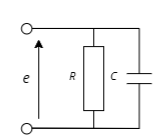
\includegraphics[width=0.4\linewidth]{./Circuits/Circuits_h.png}
            \captionof{figure}{回路h} % ✅ OK
          \end{center}
          \begin{center}
            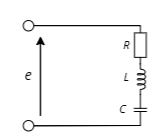
\includegraphics[width=0.4\linewidth]{./Circuits/Circuits_i.png}
            \captionof{figure}{回路i} % ✅ OK
          \end{center}
  \item (j)の回路における電力の導出
        \begin{align*}
          e               & = \sqrt{2}E\sin\omega t                                                                 \\
                          & \text{合成アドミタンスは,}                                                                       \\
          Y               & = \frac{1}{R} + \frac{1}{j\omega L} + \frac{1}{\frac{1}{j\omega C}}                     \\
                          & = \frac{1}{R} + j\left(-\frac{1}{\omega L} + \omega C\right)                            \\
          \|Y\|           & = \sqrt{{\left(\frac{1}{R}\right)}^2 + {\left(-\frac{1}{\omega L} + \omega C\right)}^2} \\
          \|Z\|           & = \frac{1}{\|Y\|}                                                                       \\
                          & \text{並列接続より各素子にかかる電圧は等しい.}                                                             \\
          i_R             & = \frac{e}{R}                                                                           \\
          ei_R            & = \sqrt{2}E\sin\omega t \cdot \frac{\sqrt{2}E}{R}\sin\omega t                           \\
                          & = \frac{2E^2}{R}\sin^2 \omega t                                                         \\
                          & = \frac{E^2}{R}\left(1 - \cos 2 \omega t\right)                                         \\
                          & \text{ここで,合成アドミタンスとの位相差を考えると}                                                           \\
                          & \frac{\frac{1}{R}}{\|Y\|} = \frac{\|Z\|}{R} = \cos \Phi\text{であるから,}                    \\
          \therefore ei_R & = \frac{E^2}{\|Z\|}\cos \Phi\left(1 - \cos 2 \omega t\right)                            \\
          &\text{次にインダクタンスによる電力を考える.}\\
          e &= L\frac{di_L}{dt}\\
          \int di_L &= \frac{1}{L} \int edt\\
          i_l &= \frac{1}{L}\int \sqrt{2}E\sin\omega t dt\\
              &= -\frac{\sqrt{2}E}{\omega L}\cos \omega t\\
          ei_L  &= \sqrt{2}E\sin\omega t \cdot -\frac{\sqrt{2}E}{\omega L}\cos \omega t\\
                &= -\frac{2E^2}{\omega L}\sin\omega t \cos \omega t\\
          &\frac{1}{2} \sin 2\alpha = \sin\alpha\cos\alpha\text{より,}\\
                &= -\frac{E^2}{\omega L}\sin 2\omega t\\
                \therefore ei_L &= -\frac{E^2}{\omega L}\sin 2\omega t\\
          &\text{最後にキャパシタンスによる電力を考える.}\\
          i_c &= \frac{de_c}{dt}C = C \frac{d}{dt}\left(\sqrt{2}E\sin\omega t\right)\\
              &= \omega C \sqrt{2}E\cos\omega t\\
          ei_c  &= \sqrt{2}E\sin \omega t \cdot \omega C \sqrt{2}E \cos \omega t\\
                &= \omega C 2 E^2 \sin \omega t \cos \omega t\\
\therefore ei_c      &= \omega C E^2 \sin 2\omega t\\
        \end{align*}

  \item (k)の回路における電力の導出
        \begin{align*}
          e &= \sqrt{2}E\sin\omega t\\
          &\text{R-L直列の合成インピーダンスを}Z_1\text{,}\\
          &Z_1\text{に流れる電流を}i_1\text{,}\\
          &\text{R-C直列の合成インピーダンスを}Z_2\text{,}\\
          &Z_2\text{に流れる電流を}i_2\text{とし}\\
          &Z_1\text{,}Z_2\text{の位相差をそれぞれ}\Phi_1 \Phi_2\\
          &\text{とすると,それぞれ以下のように示せる.}\\
          \|Z_1\| &= \sqrt{{R_1}^2 + {\left(\omega L\right)}^2}\\
          \|Z_2\| &= \sqrt{{R_2}^2 + {\left(\frac{1}{\omega C}\right)}^2}\\
          i_1 &= \frac{\sqrt{2}E}{\|Z_1\|} \sin \left(\omega t - \Phi_1\right)\\
          i_2 &= \frac{\sqrt{2}E}{\|Z_2\|} \sin \left(\omega t + \Phi_2\right)\\
          &\text{まず,}R_1\text{の電力を求める.}\\
          e_{r1} &= i_1R = \frac{\sqrt{2}ER}{\|Z_1\|}\sin\left(\omega t - \Phi_1\right)\\
          ei_{r1} &= \frac{\sqrt{2}ER}{\|Z_1\|}\sin\left(\omega t - \Phi_1\right) \cdot \frac{\sqrt{2}E}{\|Z_1\|} \sin \left(\omega t - \Phi_1\right)\\
               &= \frac{2E^2}{{\|Z_1\|}^2}R\sin^2\left(\omega t - \Phi_1\right)\\
          &\cos \Phi_1 = \frac{R}{\|Z_1\|}\text{より,}\\
               &= \frac{2E^2}{\|Z_1\|}\sin\Phi_1\sin^2\left(\omega t - \Phi_1\right)\\
\therefore ei_{r1} &= \frac{E^2}{\|Z_1\|}\sin\Phi_1 \left(1 - \cos 2 \left(\omega t - \Phi_1\right)\right)\\
          &\text{次にインダクタンスの電力を求める.}\\
          e_L &= L \frac{di_1}{dt} = L \frac{d}{dt} \left(\frac{\sqrt{2}E}{\|Z_1\|} \sin \left(\omega t - \Phi_1\right)\right)\\
              &= \frac{\sqrt{2}E}{\|Z_1\|} \omega L \cos \left( \omega t - \Phi_1 \right)\\
          &\sin \Phi_1 = \frac{\omega L}{\|Z_1\|}\text{より,}\\
              &= \sqrt{2}E\sin \Phi_1 \cos \left( \omega t - \Phi_1 \right)\\
          ei_L  &= \sqrt{2}E\sin \Phi_1 \cos \left( \omega t - \Phi_1 \right) \cdot \frac{\sqrt{2}E}{\|Z_1\|} \sin \left(\omega t - \Phi_1\right)\\
                &= \frac{2E^2}{\|Z_1\|}\sin\Phi \sin \left( \omega t - \Phi_1\right)\cos \left( \omega t - \Phi_1\right)\\
                &= \frac{E^2}{\|Z_1\|}\sin\Phi \sin2\left( \omega t - \Phi_1\right)\\
          &\text{次に,}R_2\text{の電力を求めるが,電流の位相差が異なるだけであるため,}\\
          e_{r2} &= i_2R = \frac{\sqrt{2}ER}{\|Z_2\|}\sin\left(\omega t + \Phi_2\right)\\
          ei_{r2} &= \frac{\sqrt{2}ER}{\|Z_2\|}\sin\left(\omega t + \Phi_2\right) \cdot \frac{\sqrt{2}E}{\|Z_2\|} \sin \left(\omega t + \Phi_2\right)\\          
\end{align*}
\begin{align*}
  \therefore ei_{r2} &= \frac{E^2}{\|Z_2\|}\sin\Phi_2 \left(1 - \cos 2 \left(\omega t + \Phi_2\right)\right)\\
          &\text{次に,}C\text{の電力を求める.}\\
          i_2 &= \frac{de_c}{dt}C\\
          \int de_c &= \frac{1}{C} \int di_c dt\\
          e_c   &= \frac{1}{C} \int \frac{\sqrt{2}E}{\|Z_2\|}\sin \left( \omega t + \Phi_2\right) dt\\
                &= -\frac{\sqrt{2}E}{\omega C\|Z_2\|} \cos \left( \omega t + \Phi_2\right)\\
          ei_c  &= -\frac{\sqrt{2}E}{\omega C\|Z_2\|} \cos \left( \omega t + \Phi_2\right) \cdot \frac{\sqrt{2}E}{\|Z_2\|}\sin \left( \omega t + \Phi_2\right)\\
          &\sin \Phi_2 = \frac{\omega C}{\|Z_2\|}\text{,加法定理の逆より,}\\
\therefore ei_c &= -\frac{2E^2}{\|Z_2\|}\sin \Phi_2 \sin 2\left(\omega t + \Phi_2\right)\\
          &\text{全体の電力}ei\text{は,}\\
          ei  &= e\left(i_1 + i_2\right)\\
              &= \sqrt{2}E\sin\omega t \cdot \\
              & \left(\frac{\sqrt{2}E}{\|Z_1\|}\sin\left(\omega t - \Phi_1\right) +  \frac{\sqrt{2}E}{\|Z_2\|}\sin\left(\omega t + \Phi_2\right)\right)\\
\therefore ei     =&\frac{E^2}{\|Z_1\|}\left(\cos\Phi_1 - \cos\left(2\omega t - \Phi_1\right)\right) -\\
                 &\frac{E^2}{\|Z_2\|}\left(\cos\Phi_2 + \cos\left(2\omega t + \Phi_2\right)\right)\\
\end{align*}
\begin{center}
      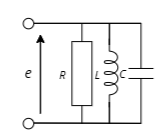
\includegraphics[width=0.4\linewidth]{./Circuits/Circuits_j.png}
      \captionof{figure}{回路j} % ✅ OK
    \end{center}
    \begin{center}
      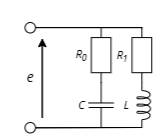
\includegraphics[width=0.4\linewidth]{./Circuits/Circuits_Z3_5.png}
      \captionof{figure}{図3.5の回路} % ✅ OK
    \end{center}
\end{enumerate}

\end{document}
